\PassOptionsToPackage{unicode=true}{hyperref} % options for packages loaded elsewhere
\PassOptionsToPackage{hyphens}{url}
%
\documentclass[]{article}
\usepackage{lmodern}
\usepackage{amssymb,amsmath}
\usepackage{ifxetex,ifluatex}
\usepackage{fixltx2e} % provides \textsubscript
\ifnum 0\ifxetex 1\fi\ifluatex 1\fi=0 % if pdftex
  \usepackage[T1]{fontenc}
  \usepackage[utf8]{inputenc}
  \usepackage{textcomp} % provides euro and other symbols
\else % if luatex or xelatex
  \usepackage{unicode-math}
  \defaultfontfeatures{Ligatures=TeX,Scale=MatchLowercase}
\fi
% use upquote if available, for straight quotes in verbatim environments
\IfFileExists{upquote.sty}{\usepackage{upquote}}{}
% use microtype if available
\IfFileExists{microtype.sty}{%
\usepackage[]{microtype}
\UseMicrotypeSet[protrusion]{basicmath} % disable protrusion for tt fonts
}{}
\IfFileExists{parskip.sty}{%
\usepackage{parskip}
}{% else
\setlength{\parindent}{0pt}
\setlength{\parskip}{6pt plus 2pt minus 1pt}
}
\usepackage{hyperref}
\hypersetup{
            pdftitle={Labo Signaalverwerking},
            pdfauthor={Dries Kennes (R0486630)},
            pdfborder={0 0 0},
            breaklinks=true}
\urlstyle{same}  % don't use monospace font for urls
\usepackage{graphicx,grffile}
\makeatletter
\def\maxwidth{\ifdim\Gin@nat@width>\linewidth\linewidth\else\Gin@nat@width\fi}
\def\maxheight{\ifdim\Gin@nat@height>\textheight\textheight\else\Gin@nat@height\fi}
\makeatother
% Scale images if necessary, so that they will not overflow the page
% margins by default, and it is still possible to overwrite the defaults
% using explicit options in \includegraphics[width, height, ...]{}
\setkeys{Gin}{width=\maxwidth,height=\maxheight,keepaspectratio}
\setlength{\emergencystretch}{3em}  % prevent overfull lines
\providecommand{\tightlist}{%
  \setlength{\itemsep}{0pt}\setlength{\parskip}{0pt}}
\setcounter{secnumdepth}{0}
% Redefines (sub)paragraphs to behave more like sections
\ifx\paragraph\undefined\else
\let\oldparagraph\paragraph
\renewcommand{\paragraph}[1]{\oldparagraph{#1}\mbox{}}
\fi
\ifx\subparagraph\undefined\else
\let\oldsubparagraph\subparagraph
\renewcommand{\subparagraph}[1]{\oldsubparagraph{#1}\mbox{}}
\fi

% set default figure placement to htbp
\makeatletter
\def\fps@figure{htbp}
\makeatother


\title{Labo Signaalverwerking}
\author{Dries Kennes (R0486630)}
\date{}

\begin{document}
\maketitle

\hypertarget{header-n5299}{%
\section{Opdracht 2A: Analyse v.e. actieve
filtertrap}\label{header-n5299}}

\hypertarget{header-n5300}{%
\subsection{Opgave}\label{header-n5300}}

\begin{figure}
\centering
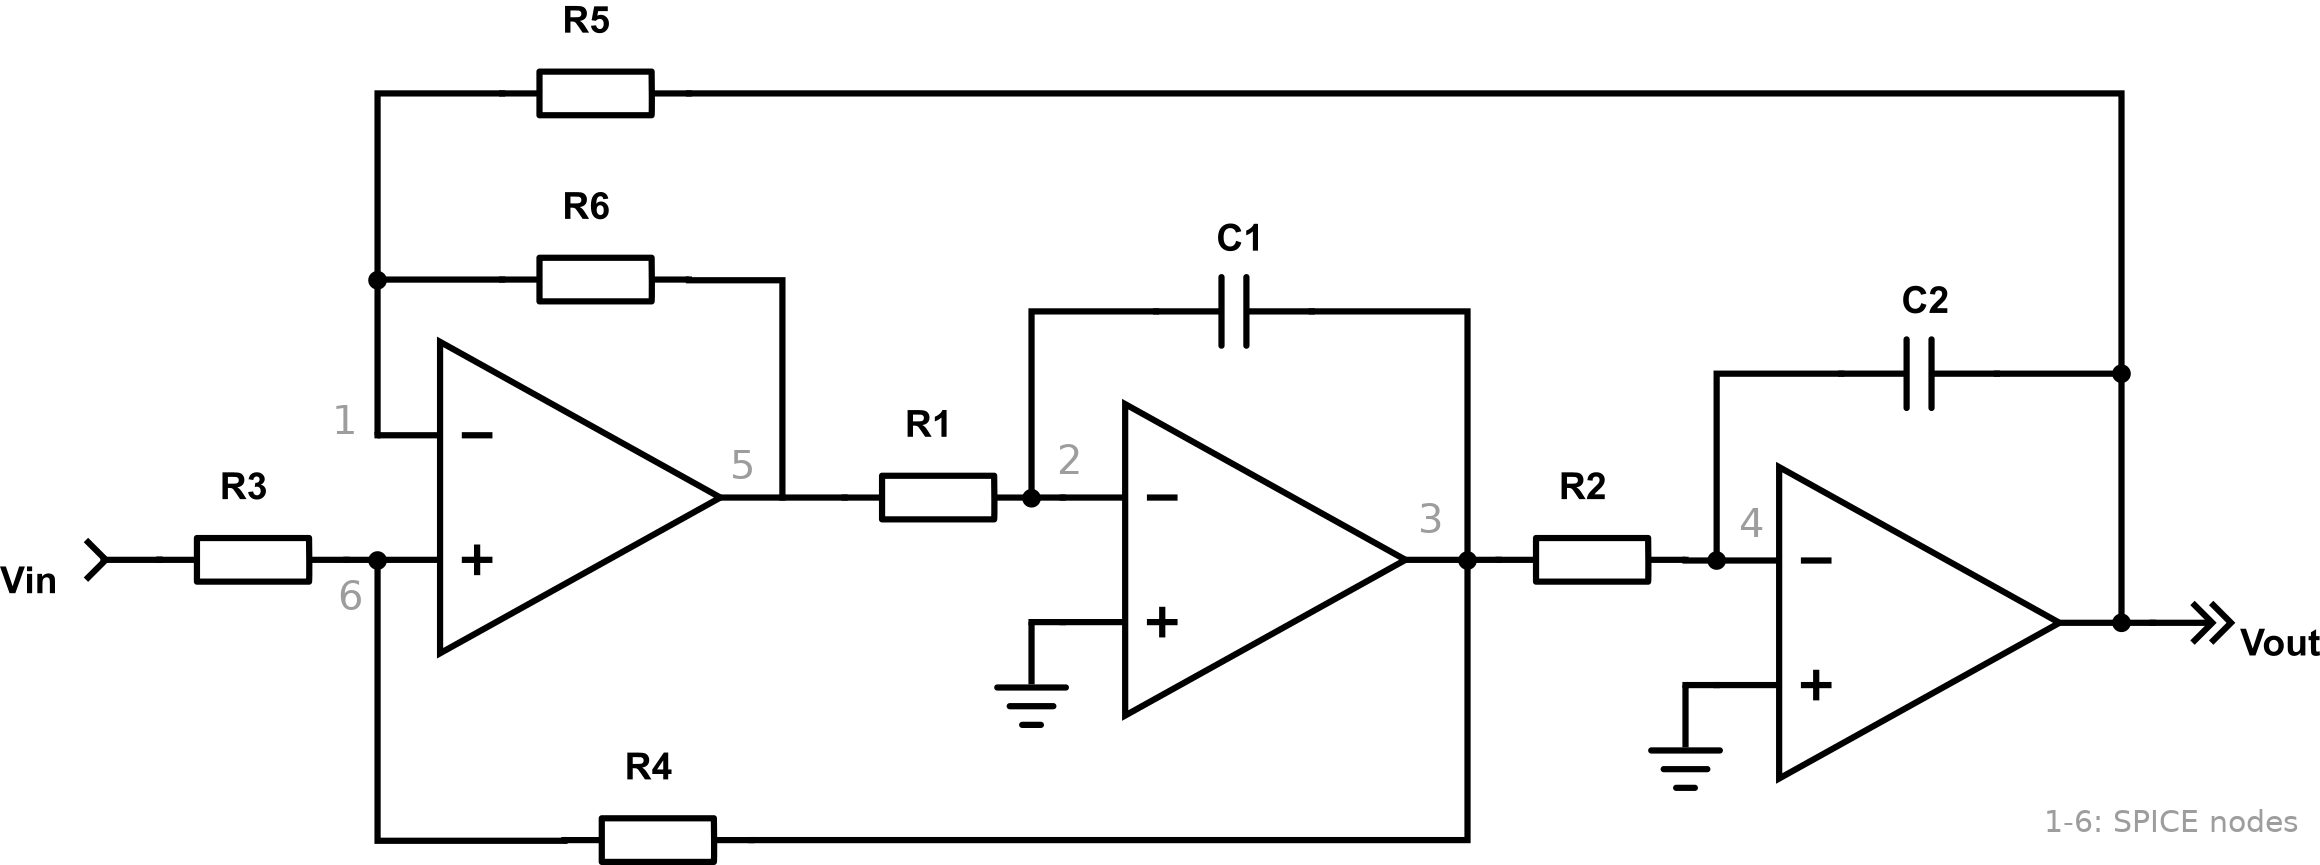
\includegraphics{/home/dries/Projects/Signaalverwerking/assets/AF_05_LP_KHNni.png}
\caption{Het schema.}
\end{figure}

\begin{itemize}
\item
  \textbf{Low Pass KHN - Non Inverting} (schema nr 5)
\item
  Filter is een \emph{LDL}

  \begin{itemize}
  \item
    \(|H(0)| = 6dB\)
  \item
    \(|H(10 kHz)| = -34dB\)
  \item
    \(Q_p = 4\)
  \end{itemize}
\end{itemize}

\hypertarget{header-n5320}{%
\subsection{Analyse}\label{header-n5320}}

\hypertarget{header-n5321}{%
\subsubsection{1. Bepaal de DC- en HF-weergave}\label{header-n5321}}

\hypertarget{header-n5322}{%
\paragraph{DC}\label{header-n5322}}

Bij DC zijn condensatoren open kring, dus wordt de versterking bepaald
door de feedback weerstanden \(R_4\), \(R_5\), en \(R_6\). Dit is dus
een vaste versterking. \(|H(DC)| = A\).

\begin{figure}
\centering
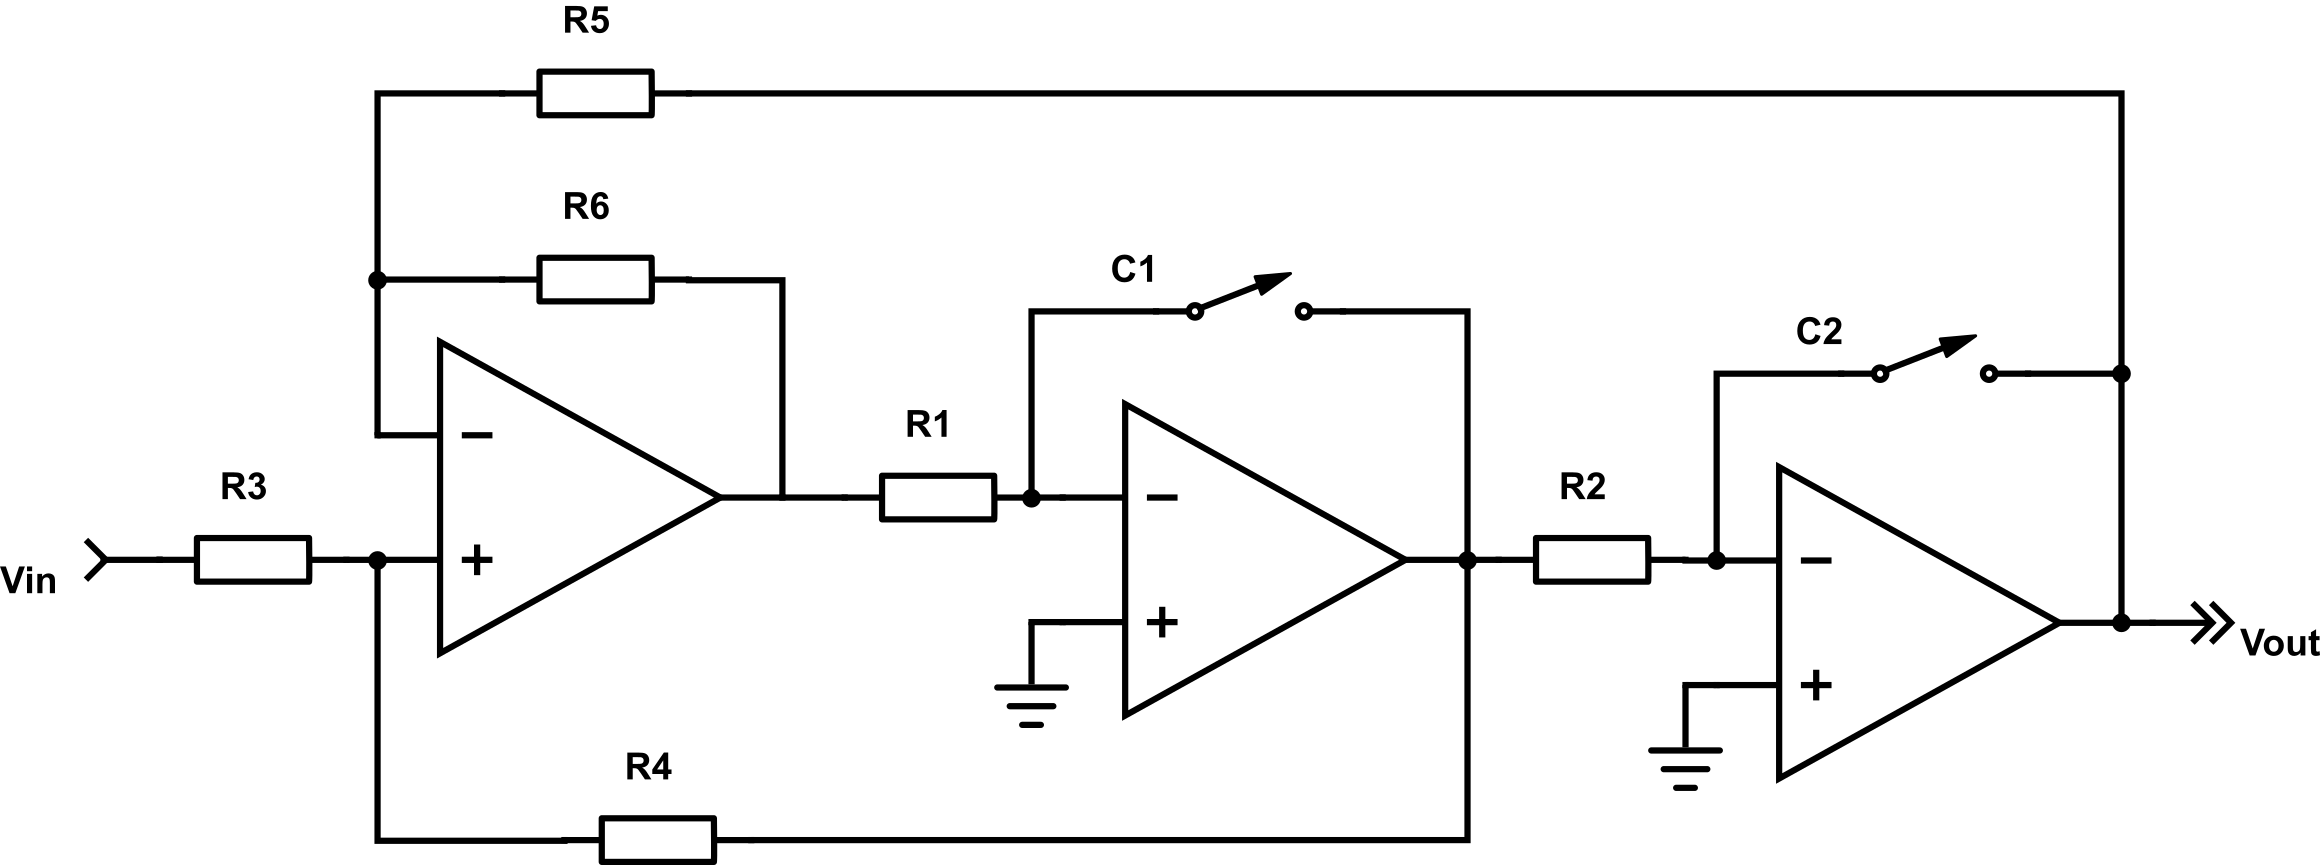
\includegraphics{/home/dries/Projects/Signaalverwerking/assets/AF_05_LP_KHNni_DC.png}
\caption{Schema met alle condensatoren open kring.}
\end{figure}

\hypertarget{header-n5327}{%
\paragraph{HF}\label{header-n5327}}

Bij HF (\(f=\infty\)) zijn de condensatoren kortsluitingen, dus wordt
het signaal volledig onderdrukt door de feedback lussen \(C_1\) en
\(C_2\). \(|H(HF)| = -\infty dB\)

\begin{figure}
\centering
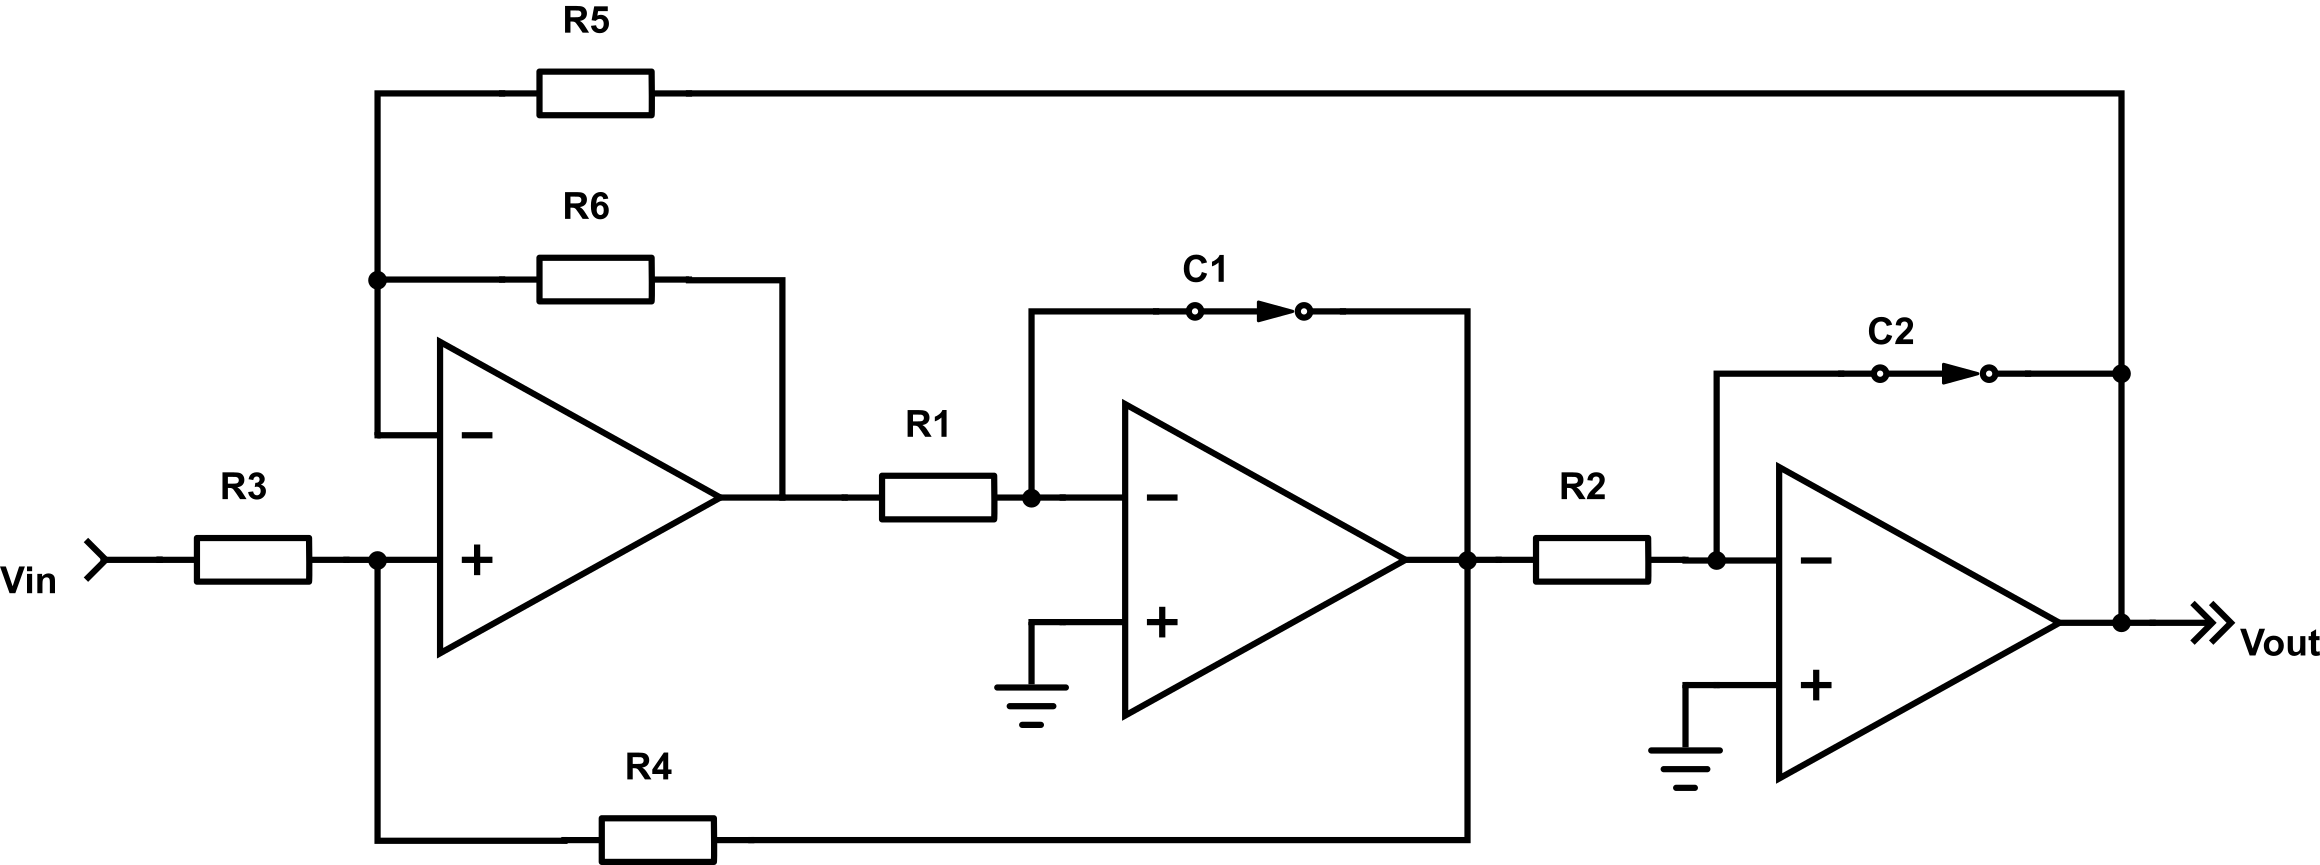
\includegraphics{/home/dries/Projects/Signaalverwerking/assets/AF_05_LP_KHNni_HF.png}
\caption{Schema met alle condensatoren kortgesloten.}
\end{figure}

\hypertarget{header-n5332}{%
\subsubsection{2. Bepaal de transferfunctie}\label{header-n5332}}

Ik heb de transfer functie uitgerekend door het schema op te splitsen in
twee integrators en de eerste opamp.

\hypertarget{header-n5335}{%
\paragraph{De integrators}\label{header-n5335}}

\begin{figure}
\centering
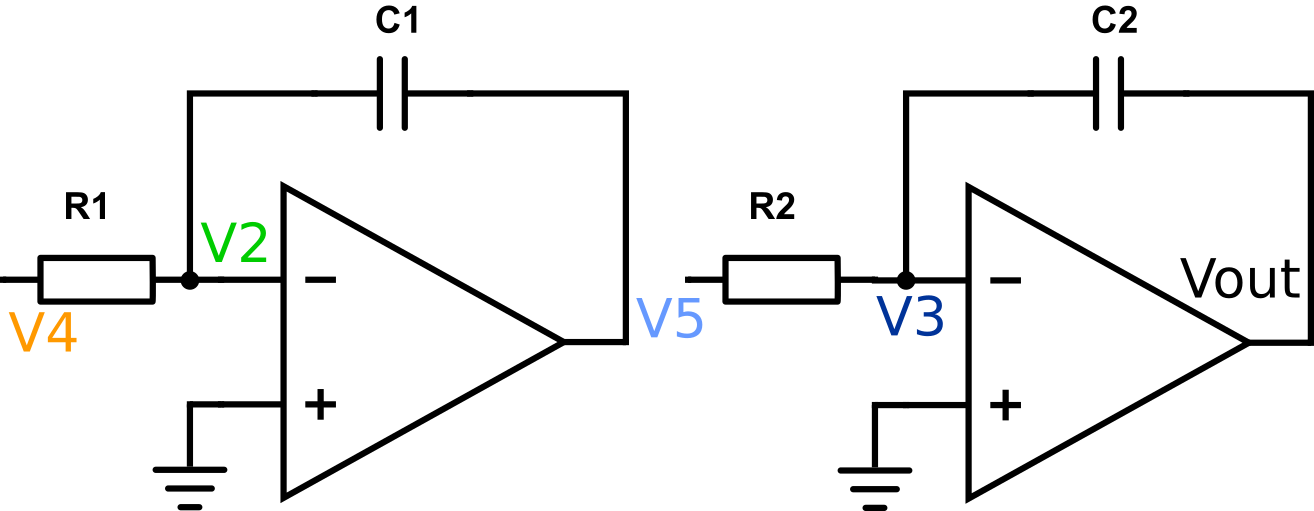
\includegraphics{/home/dries/Projects/Signaalverwerking/assets/integrators.png}
\caption{Deel van het schema met de integrators.}
\end{figure}

De algemene formule voor een integrator is \(v_o=\frac{-v_1}{sRC}\).\\
Voor deze twee specifieke gevallen: \(v_5=\frac{-v_4}{sR_1C_1}\) en
\(v_{out} = \frac{-v_5}{sR_2C_2}\).\\
Gecombineerd: \(v_{out}=\frac{v_4}{s^2R_1C_1R_2C_2} \) of
\(v_4 = s^2R_1R_2C_1C_2v_{out}\)

\hypertarget{header-n5342}{%
\paragraph{Superpositie}\label{header-n5342}}

\hypertarget{header-n5343}{%
\subparagraph{\texorpdfstring{Geval 1: \(v_{in}\),
\(v_{out} = v_5 = 0\)}{Geval 1: v\_\{in\}, v\_\{out\} = v\_5 = 0}}\label{header-n5343}}

\begin{figure}
\centering
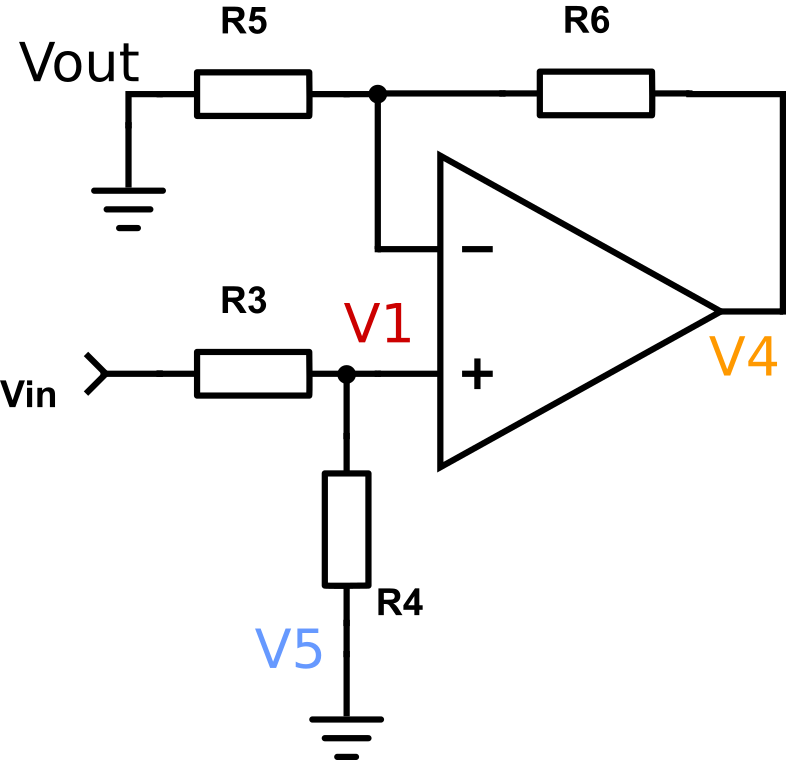
\includegraphics{/home/dries/Projects/Signaalverwerking/assets/superpositie1.png}
\caption{Superpositie schema geval 1}
\end{figure}

De opamp is nu een niet inverterende versterker. \\
\(v_4 = v_1 \cdot (1+\frac{R_6}{R_5})\)\\
\(v_1 = v_{in} \cdot \frac{R_4}{R_3+R_4} \Rightarrow v_4 = v_{in} \cdot \frac{R_4}{R_3+R_4} \cdot (1+\frac{R_6}{R_5}) = v_{in} \cdot \frac{R_4}{R_3+R_4} \cdot \frac{R_6+R_5}{R_5}\)

\hypertarget{header-n5350}{%
\subparagraph{\texorpdfstring{Geval 2: \(v_5\),
\(v_{out} = v_{in} = 0\)}{Geval 2: v\_5, v\_\{out\} = v\_\{in\} = 0}}\label{header-n5350}}

\begin{figure}
\centering
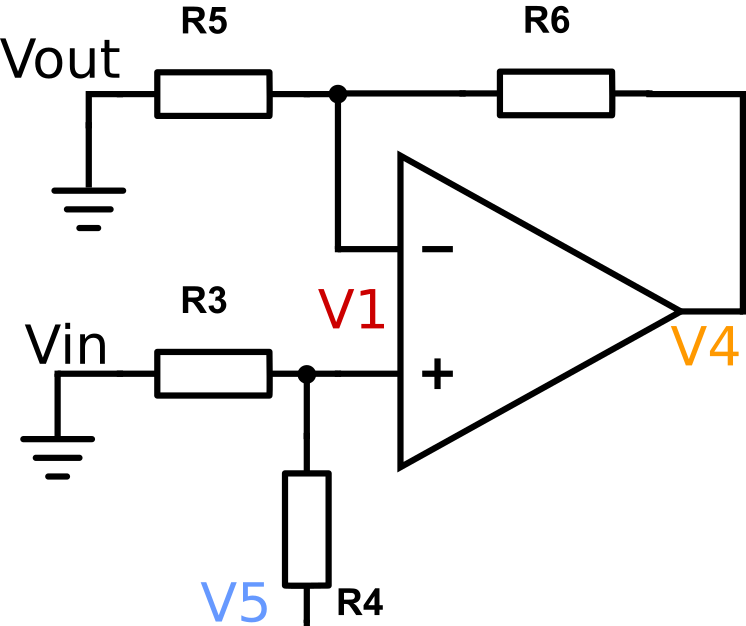
\includegraphics{/home/dries/Projects/Signaalverwerking/assets/superpositie2.png}
\caption{Superpositie schema geval 2}
\end{figure}

De opamp is nu een niet inverterende versterker.

\(v_4 = v_1 \cdot (1+\frac{R_6}{R_5})\)\\
\(v_1 = v_5 \cdot \frac{R_3}{R_3+R_4} \Rightarrow v_4 = v_5 \cdot \frac{R_3}{R_3+R_4} \cdot (1+\frac{R_6}{R_5}) = v_5 \cdot \frac{R_3}{R_3+R_4} \cdot \frac{R_6+R_5}{R_5}\)

\hypertarget{header-n5358}{%
\subparagraph{\texorpdfstring{Geval 3: \(v_{out}\),
\(v_5 = v_{in} = 0\)}{Geval 3: v\_\{out\}, v\_5 = v\_\{in\} = 0}}\label{header-n5358}}

\begin{figure}
\centering
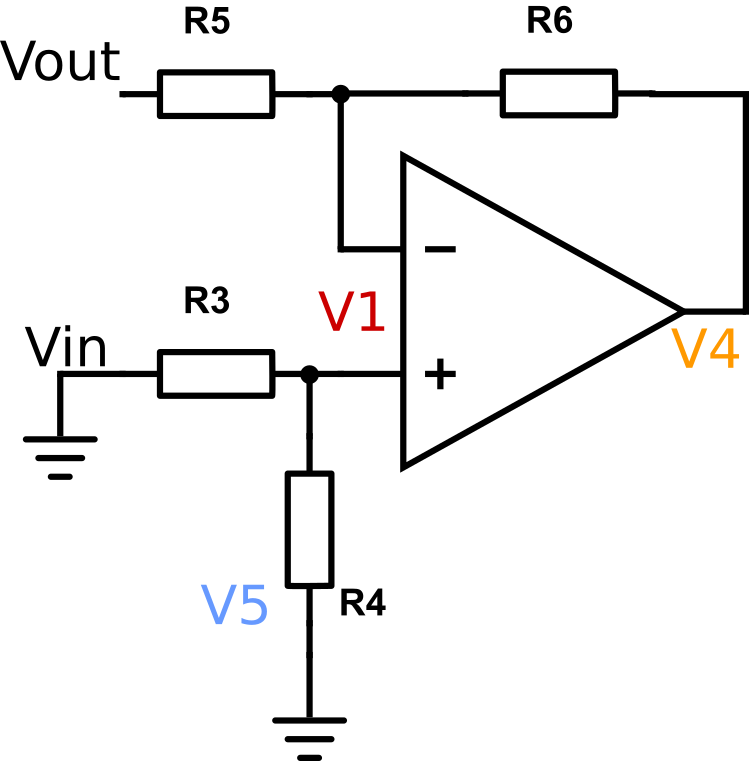
\includegraphics{/home/dries/Projects/Signaalverwerking/assets/superpositie3.png}
\caption{Superpositie schema geval 3}
\end{figure}

De opamp is nu een inverterende versterker.

\(v_4 = \frac{-R_6}{R5} \cdot v_{out}\)

\hypertarget{header-n5365}{%
\paragraph{Totaal}\label{header-n5365}}

\(v_4 = \sum{v_4} = v_{in} \cdot \frac{R_4}{R_3+R_4} \cdot \frac{R_6+R_5}{R_5} + v_5 \cdot \frac{R_3}{R_3+R_4} \cdot \frac{R_6+R_5}{R_5} + \frac{-R_6}{R5} \cdot v_{out}\)

\(v_{in} \cdot \frac{R_4}{R_3+R_4} \cdot \frac{R_6+R_5}{R_5} = -v_5 \cdot \frac{R_3}{R_3+R_4} \cdot \frac{R_6+R_5}{R_5} + \frac{R_6}{R5} \cdot v_{out} + v_4\)

Vervang in deze formule \(v_5\) en \(v_4\) door de formules van de twee
integrators:

\(v_{in} \cdot \frac{R_4}{R_3+R_4} \cdot \frac{R_6+R_5}{R_5} = v_{out} \cdot (sR_2C_2 \cdot \frac{R_3}{R_3+R_4} \cdot \frac{R_6+R_5}{R_5} + \frac{R_6}{R5} + s^2R_1R_2C_1C_2v)\)

\(\frac{v_{in}}{v_{out}} \cdot \frac{R_4}{R_3+R_4} \cdot \frac{R_6+R_5}{R_5} = s^2R_1R_2C_1C_2 + sR_2C_2 \cdot \frac{R_3}{R_3+R_4} \cdot \frac{R_6+R_5}{R_5} + \frac{R_6}{R5}\)

\(\frac{v_{out}}{v_{in}} = \frac{R_4}{R_3+R_4} \cdot \frac{R_6+R_5}{R_5} \cdot \frac{1}{s^2R_1R_2C_1C_2 + sR_2C_2 \cdot \frac{R_3}{R_3+R_4} \cdot \frac{R_6+R_5}{R_5} + \frac{R_6}{R5}}\)

\(\frac{v_{out}}{v_{in}} = \frac{R_4}{R_3+R_4} \cdot \frac{R_6+R_5}{R_5} \cdot \frac{1}{\frac{R_6}{R5} \cdot (s^2 \cdot \frac{R_1R_2C_1C_2R_5}{R_6} + sR_2C_2 \cdot \frac{R_3}{R_3+R_4} \cdot \frac{R_6+R_5}{R_6} + 1)}\)

Het resultaat:
\(H(s) = \frac{v_{out}}{v_{in}} = \frac{R_4}{R_3+R_4} \cdot \frac{R_6+R_5}{R_6} \cdot \frac{1}{s^2 \cdot \frac{R_1R_2C_1C_2R_5}{R_6} + sR_2C_2 \cdot \frac{R_3}{R_3+R_4} \cdot \frac{R_6+R_5}{R_6} + 1}\)

\hypertarget{header-n5382}{%
\subsubsection{3. Vergelijk transfer functie met de
algemene}\label{header-n5382}}

Geen teller, dus geen zeros, enkel polen.

Algemene vorm LDL filter:
\(H(s) = K\frac{1}{(\frac{s}{\omega_n})^2+\frac{1}{Q}\cdot(\frac{s}{\omega_n})+1}\)

\begin{itemize}
\item
  \(K=\frac{R_4}{R_3+R_4} \cdot \frac{R_5+R_6}{R_6}\)
\item
  \(\frac{1}{\omega_n^2} = \frac{C_1C_2R_1R_2R_5}{R_6}\)
\item
  \(\frac{1}{Q\omega_n}=C_2R_2 \cdot \frac{R_3}{R_4+R_3} \cdot \frac{R_5+R_6}{R_6}\)
\end{itemize}

Kies:

\begin{itemize}
\item
  \(C_2 = c^{te} = 1\)\\
  Kies \(C_2\) omdat van \(C_1\) makkelijker een ontwerpvergelijking te
  vinden is.
\item
  \(R = R_1 = R_2 = R_3 = R_4 = R_6\)\\
  \(R_5\) variabel omdat die enkel in tellers zit. Dit maakt
  ontwerpvergelijkingen makkelijker.
\end{itemize}

Dit maakt dan

\begin{itemize}
\item
  \(K = \frac{R+R_5}{2R}\)
\item
  \(\frac{1}{\omega_n^2} = C_1C_2RR_5\)
\item
  \(\frac{1}{Q\omega_n}=\frac{C_2(R+R_5)}{2}\)
\end{itemize}

Transfer functie met componenten:
\(H(s) = \frac{R+R_5}{2R} \cdot \frac{1}{s^2C_1C_2RR_5+s\frac{C2(R+R_5)}{2}+1}\)

\hypertarget{header-n5420}{%
\subsection{Synthese}\label{header-n5420}}

\hypertarget{header-n5421}{%
\subsubsection{1. Ontwerpvergelijkingen}\label{header-n5421}}

\begin{itemize}
\item
  \(K = \frac{R+R_5}{2R} \Rightarrow R + R_5 = 2RK\) and
  \(\frac{1}{Q\omega_n} = \frac{C_2(R+R_5)}{2} = C_2RK \Rightarrow R = \frac{1}{C_2KQ\omega_n}\)
\item
  \(R+R_5 = 2KR \Rightarrow R_5 = (2K-1)R \Rightarrow R_5 = \frac{2K-1}{C_2KQ\omega_n}\)
\item
  \(\omega_n^2=\frac{1}{C_1C_2RR_5} \Rightarrow C_1 = \frac{1}{C_2RR_5\omega_n^2}\)
\end{itemize}

\hypertarget{header-n5432}{%
\subsubsection{2. Impedantieschaling}\label{header-n5432}}

Schalingsfactor: 10\textsuperscript{6}

\end{document}
